\documentclass{siproblemset}

% SI Session Information
\course{MTH 1321}       % the course of your SI
\sessionnum{23}         % (optional) specify the session number
\sessiondate{12/4/19}   % the date of the session

\warmup{Concept Review}
\topic{Fundamental Theorem of Calculus, Part II}
\topic{Net Change as Integrals of Rates of Change}
\topic{$u$-substitution}

% Worksheet Information
\title{FTOCII, Net Change,\linebreak $u$-substitution}
\sections{Sections 5.5--5.7}
\withnamespace

\newcommand{\dx}{\text{d}x}

\begin{document}
    \maketitle
    
    \activity{Warmup}{Concept Review}{Work \textbf{alone} to answer these questions. Try not to use your notes.}{15 minutes}
    
    \frq{What is the Fundamental Theorem of Calculus, Part II?}
    \smallsp
    
    \frq{What is distance? What is displacement? Given the velocity function $v(t)$, construct an integral to find both quantities on the interval $t=[0\text s,5\text s]$.}
    \Normalsp
    
    \frq{What are the steps to solve a $u$-substitution problem?}
   
    \newpage
   
    \activity{Activity 1}{Fundamental Theorem of Calculus, Part II}{Make a \textbf{group of two or three, all with the same colored worksheets}, to work together to answer these questions. Try not to use your notes. \textbf{DO NOT use a calculator}.}{30 minutes}
    \mcq{Find the formula for the are function represented by the following integrals.}{
        \task $\int_{4}^{x}e^{3u}\dd u$
        \normalsp
        \task $\int_{x}^{0}2^{-t}\dd t$
        \normalsp
    }
    \mcq{Compute the following derivatives.}{
        \task $\dddf t\int_{0}^{t}x^4-7x^2\dx$
        \normalsp
        \task $\dddf s\int_{100}^{s}\ln(6u-5)\dd u$
        \normalsp
    }
    \mcq{Compute the following derivatives.}{
        \task $\dddf x\int_{0}^{x^2}\frac{t\dd t}{t+1}$
        \Normalsp
        \task $\dddf t\int_{-4}^{\sec(t)}u^3\dd u$
        \Normalsp
    }
    \newpage
    \activity{Activity 2}{Net Change as Integrals of Rates of Change}{Make a \textbf{group of two or three, all with the same colored worksheets}, to work together to do your assigned parts. Then, try to do the other parts. Try not to use your notes. \textbf{DO NOT use a calculator}.}{30 minutes}
    
    \frq{A survey shoes that a candidate is gaining votes at a rate of $2000t+1000$ votes per day, where $t$ is the number of days since she announced her candidacy. How many supporters will the candidate have after 60 days (assuming that she had no supporters at $t=0$)?}
    \Largesp
    \frq{The traffic flow rate past a certain point on a highway is $q(t)=3000+2000t-300t^2$ ($t$ is in hours), where $t=0$ is 8am. How many cars pass by in the time interval from 8 to 10am?}
    \newpage
    \frq{A particle moves in a straight line with velocity $v(t)=t^{-2}-1$ m/s. Find the displacement and total distance traveled over the time interval $[0.5,2]$ seconds.}
    \Normalsp
    \frq{Find the distance and displacement of a person whose velocity $v$ as a piecewise function of time $t$ is shown below. Show the integrals that you will use to compute this, then compute geometrically.}
    \begin{center}
        \mbox{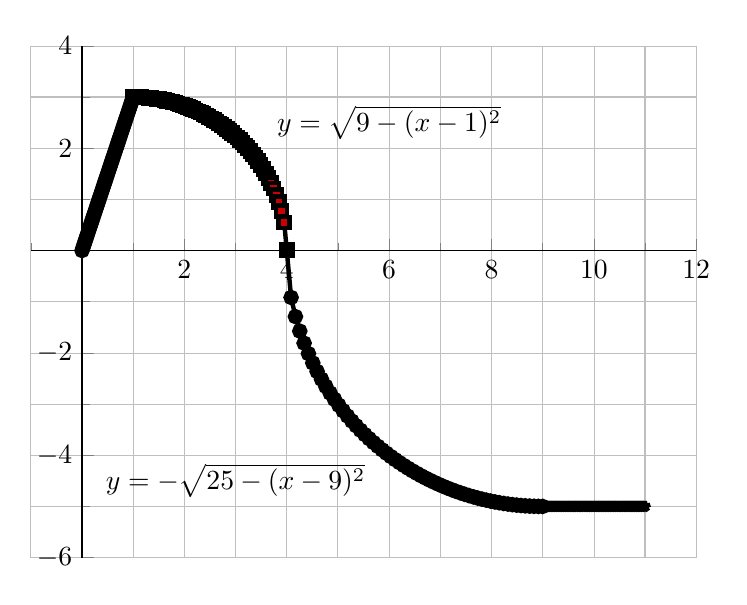
\begin{tikzpicture}[baseline=(current bounding box.north)]
            \begin{axis}[
            x=0.65cm,
            y=0.65cm,
            xmin=-1,
            xmax=12,
            ymin=-6,
            ymax=4,
            grid=both,
            major grid style={line width=.2pt,draw=gray!50},
            minor tick num=1,
            axis x line*=middle,
            axis y line*=middle,
            every axis plot/.append style={ultra thick},
            samples=60
            ]
            \addplot+[black, domain=0:1] {3*x};
            \addplot+[black, domain=1:4] {sqrt(9-(x-1)^2)};
            \node at (6,2.5) {$y=\sqrt{9-(x-1)^2}$};
            \addplot+[black, domain=4:9] {-sqrt(25-(x-9)^2)};
            \node at (3,-4.5) {$y=-\sqrt{25-(x-9)^2}$};
            \addplot+[black, domain=9:11] {-5};
            \end{axis}
            \end{tikzpicture}}
        
        Graph of $v(t)$
    \end{center}
    \newpage
    
    \activity{Activity 3}{$u$-substitution}{Make a \textbf{group of two or three, all with the same colored worksheets}, to work together to do your assigned parts. Then, try to do the other parts. Try not to use your notes. \textbf{DO NOT use a calculator}.}{30 minutes}
        
    \mcq{Compute the following indefinite integrals.}{
        \task $\int\frac{\dx}{\sqrt{x}\paren{1+\sqrt{x}}^2}$
        \Smallsp
        \task $\int\sec^2(\theta)\tan(\theta)\dd\theta$
        \Smallsp
        \task $\int\sqrt{4x-1}\dx$
        \Smallsp
        \task $\int t\sqrt{4t-1}\dd t$
        \Smallsp
    }

    \mcq{Compute the following definite integrals.}{
        \task $\int_{-8/3}^{-2}(3x+8)^{11}\dx$
        \Smallsp
        \task $\int_{1}^{2}\frac{t\dd t}{\sqrt{t^2+9}}$
        \Smallsp
        \task $\int_{\arcsin{(\pi/4)}}^{\arcsin{(\pi/2)}}\cos(\theta)\cos(\sin(\theta))\dd\theta$
        \Smallsp
        \task $\int_{1}^{2}xe^{x^2}\dx$
        \Smallsp
    }
\end{document}